\documentclass{standalone}
\usepackage{graphicx}	
\usepackage{amssymb, amsmath}
\usepackage{color}
\usepackage{wasysym}

\usepackage{tikz}
\usetikzlibrary{intersections, backgrounds}
\usepackage{pgfmath}

\definecolor{light}{RGB}{220, 188, 188}
\definecolor{mid}{RGB}{185, 124, 124}
\definecolor{dark}{RGB}{143, 39, 39}
\definecolor{highlight}{RGB}{180, 31, 180}
\definecolor{gray10}{gray}{0.1}
\definecolor{gray20}{gray}{0.2}
\definecolor{gray30}{gray}{0.3}
\definecolor{gray40}{gray}{0.4}
\definecolor{gray60}{gray}{0.6}
\definecolor{gray70}{gray}{0.7}
\definecolor{gray80}{gray}{0.8}
\definecolor{gray90}{gray}{0.9}
\definecolor{gray95}{gray}{0.95}

\newcommand*{\offset}{0.025}

\begin{document}

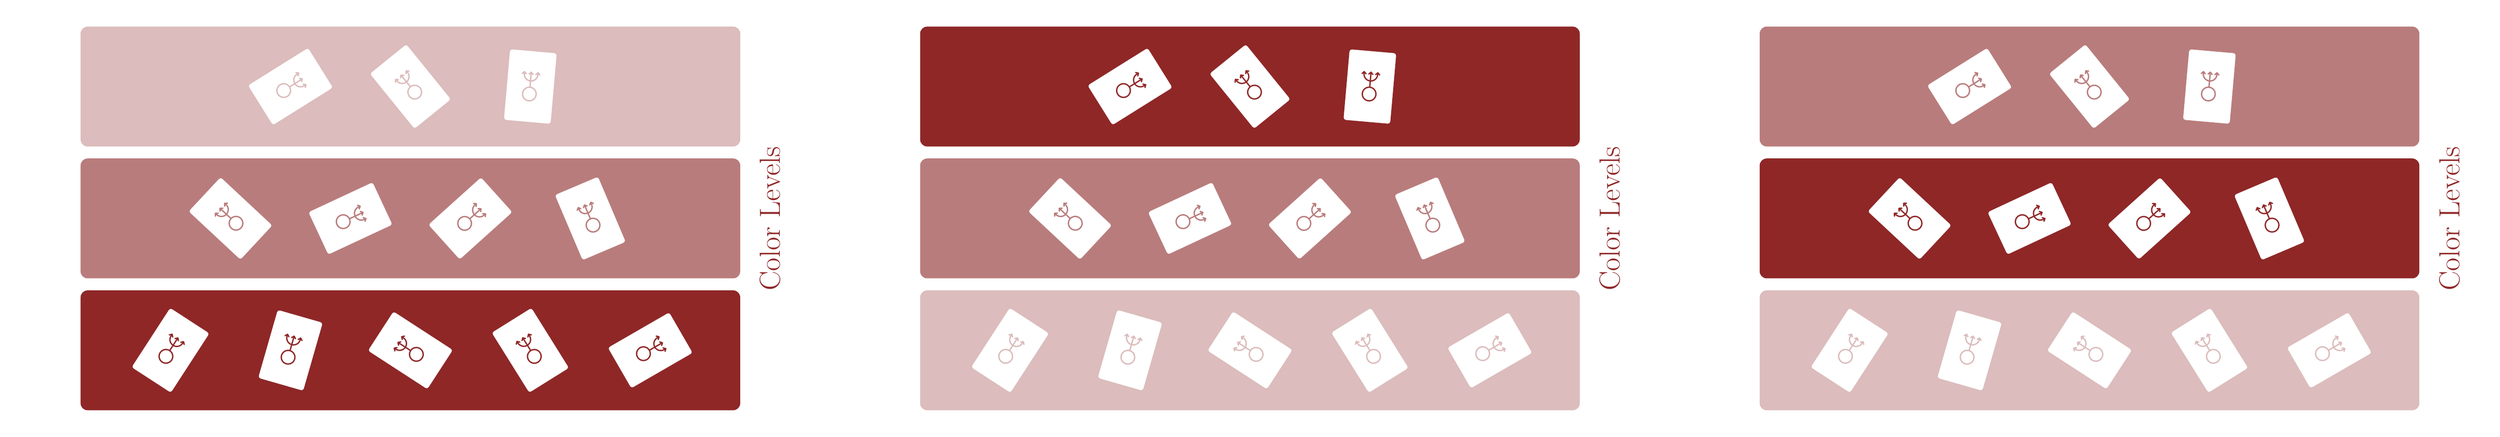
\begin{tikzpicture}[scale=0.3, thick]

\pgfmathsetmacro{\cx}{2}
\pgfmathsetmacro{\cy}{3}


\begin{scope}

\draw[white] (-33, -17) rectangle (33, 17);

\node[dark, rotate=90] at (30, 0) { \huge Color Levels };

\fill[light, rounded corners=5] (-27.5, 11 - 5) rectangle (27.5, 11 + 5);
\fill[mid, rounded corners=5] (-27.5, 0 - 5) rectangle (27.5, 0 + 5);
\fill[dark, rounded corners=5] (-27.5, -11 - 5) rectangle (27.5, -11 + 5);

% Row One
\pgfmathsetmacro{\phi}{-58}
\pgfmathsetmacro{\x}{-10}
\pgfmathsetmacro{\y}{11}
\begin{scope}[shift={(\x, \y)}, rotate={\phi}]
  \filldraw[fill=white, draw=light, rounded corners=2] (0 - \cx, 0 - \cy) rectangle (0 + \cx, 0 + \cy);
  \node[light, rotate={\phi}] at (0.17, 0) { $\Huge \neptune$ }; 
\end{scope}

\pgfmathsetmacro{\phi}{39}
\pgfmathsetmacro{\x}{0}
\pgfmathsetmacro{\y}{11}
\begin{scope}[shift={(\x, \y)}, rotate={\phi}]
  \filldraw[fill=white, draw=light, rounded corners=2] (0 - \cx, 0 - \cy) rectangle (0 + \cx, 0 + \cy);
  \node[light, rotate={\phi}] at (0.17, 0) { $\Huge \neptune$ }; 
\end{scope}

\pgfmathsetmacro{\phi}{-5}
\pgfmathsetmacro{\x}{10}
\pgfmathsetmacro{\y}{11}
\begin{scope}[shift={(\x, \y)}, rotate={\phi}]
  \filldraw[fill=white, draw=light, rounded corners=2] (0 - \cx, 0 - \cy) rectangle (0 + \cx, 0 + \cy);
  \node[light, rotate={\phi}] at (0.17, 0) { $\Huge \neptune$ }; 
\end{scope}

% Row Two
\pgfmathsetmacro{\phi}{47}
\pgfmathsetmacro{\x}{-15}
\pgfmathsetmacro{\y}{0}
\begin{scope}[shift={(\x, \y)}, rotate={\phi}]
  \filldraw[fill=white, draw=mid, rounded corners=2] (0 - \cx, 0 - \cy) rectangle (0 + \cx, 0 + \cy);
  \node[mid, rotate={\phi}] at (0.17, 0) { $\Huge \neptune$ }; 
\end{scope}

\pgfmathsetmacro{\phi}{-65}
\pgfmathsetmacro{\x}{-5}
\pgfmathsetmacro{\y}{0}
\begin{scope}[shift={(\x, \y)}, rotate={\phi}]
  \filldraw[fill=white, draw=mid, rounded corners=2] (0 - \cx, 0 - \cy) rectangle (0 + \cx, 0 + \cy);
  \node[mid, rotate={\phi}] at (0.17, 0) { $\Huge \neptune$ }; 
\end{scope}

\pgfmathsetmacro{\phi}{-48}
\pgfmathsetmacro{\x}{5}
\pgfmathsetmacro{\y}{0}
\begin{scope}[shift={(\x, \y)}, rotate={\phi}]
  \filldraw[fill=white, draw=mid, rounded corners=2] (0 - \cx, 0 - \cy) rectangle (0 + \cx, 0 + \cy);
  \node[mid, rotate={\phi}] at (0.17, 0) { $\Huge \neptune$ }; 
\end{scope}

\pgfmathsetmacro{\phi}{23}
\pgfmathsetmacro{\x}{15}
\pgfmathsetmacro{\y}{0}
\begin{scope}[shift={(\x, \y)}, rotate={\phi}]
  \filldraw[fill=white, draw=mid, rounded corners=2] (0 - \cx, 0 - \cy) rectangle (0 + \cx, 0 + \cy);
  \node[mid, rotate={\phi}] at (0.17, 0) { $\Huge \neptune$ }; 
\end{scope}

% Row Three
\pgfmathsetmacro{\phi}{-33}
\pgfmathsetmacro{\x}{-20}
\pgfmathsetmacro{\y}{-11}
\begin{scope}[shift={(\x, \y)}, rotate={\phi}]
  \filldraw[fill=white, draw=dark, rounded corners=2] (0 - \cx, 0 - \cy) rectangle (0 + \cx, 0 + \cy);
  \node[dark, rotate={\phi}] at (0.17, 0) { $\Huge \neptune$ }; 
\end{scope}

\pgfmathsetmacro{\phi}{-16}
\pgfmathsetmacro{\x}{-10}
\pgfmathsetmacro{\y}{-11}
\begin{scope}[shift={(\x, \y)}, rotate={\phi}]
  \filldraw[fill=white, draw=dark, rounded corners=2] (0 - \cx, 0 - \cy) rectangle (0 + \cx, 0 + \cy);
  \node[dark, rotate={\phi}] at (0.17, 0) { $\Huge \neptune$ }; 
\end{scope}

\pgfmathsetmacro{\phi}{57}
\pgfmathsetmacro{\x}{0}
\pgfmathsetmacro{\y}{-11}
\begin{scope}[shift={(\x, \y)}, rotate={\phi}]
  \filldraw[fill=white, draw=dark, rounded corners=2] (0 - \cx, 0 - \cy) rectangle (0 + \cx, 0 + \cy);
  \node[dark, rotate={\phi}] at (0.17, 0) { $\Huge \neptune$ }; 
\end{scope}

\pgfmathsetmacro{\phi}{32}
\pgfmathsetmacro{\x}{10}
\pgfmathsetmacro{\y}{-11}
\begin{scope}[shift={(\x, \y)}, rotate={\phi}]
  \filldraw[fill=white, draw=dark, rounded corners=2] (0 - \cx, 0 - \cy) rectangle (0 + \cx, 0 + \cy);
  \node[dark, rotate={\phi}] at (0.17, 0) { $\Huge \neptune$ }; 
\end{scope}

\pgfmathsetmacro{\phi}{-60}
\pgfmathsetmacro{\x}{20}
\pgfmathsetmacro{\y}{-11}
\begin{scope}[shift={(\x, \y)}, rotate={\phi}]
  \filldraw[fill=white, draw=dark, rounded corners=2] (0 - \cx, 0 - \cy) rectangle (0 + \cx, 0 + \cy);
  \node[dark, rotate={\phi}] at (0.17, 0) { $\Huge \neptune$ }; 
\end{scope}

\end{scope}



\begin{scope}[shift={(70, 0)}]

\draw[white] (-33, -17) rectangle (33, 17);

\node[dark, rotate=90] at (30, 0) { \huge Color Levels };

\fill[dark, rounded corners=5] (-27.5, 11 - 5) rectangle (27.5, 11 + 5);
\fill[mid, rounded corners=5] (-27.5, 0 - 5) rectangle (27.5, 0 + 5);
\fill[light, rounded corners=5] (-27.5, -11 - 5) rectangle (27.5, -11 + 5);

% Row One
\pgfmathsetmacro{\phi}{-58}
\pgfmathsetmacro{\x}{-10}
\pgfmathsetmacro{\y}{11}
\begin{scope}[shift={(\x, \y)}, rotate={\phi}]
  \filldraw[fill=white, draw=dark, rounded corners=2] (0 - \cx, 0 - \cy) rectangle (0 + \cx, 0 + \cy);
  \node[dark, rotate={\phi}] at (0.17, 0) { $\Huge \neptune$ }; 
\end{scope}

\pgfmathsetmacro{\phi}{39}
\pgfmathsetmacro{\x}{0}
\pgfmathsetmacro{\y}{11}
\begin{scope}[shift={(\x, \y)}, rotate={\phi}]
  \filldraw[fill=white, draw=dark, rounded corners=2] (0 - \cx, 0 - \cy) rectangle (0 + \cx, 0 + \cy);
  \node[dark, rotate={\phi}] at (0.17, 0) { $\Huge \neptune$ }; 
\end{scope}

\pgfmathsetmacro{\phi}{-5}
\pgfmathsetmacro{\x}{10}
\pgfmathsetmacro{\y}{11}
\begin{scope}[shift={(\x, \y)}, rotate={\phi}]
  \filldraw[fill=white, draw=dark, rounded corners=2] (0 - \cx, 0 - \cy) rectangle (0 + \cx, 0 + \cy);
  \node[dark, rotate={\phi}] at (0.17, 0) { $\Huge \neptune$ }; 
\end{scope}

% Row Two
\pgfmathsetmacro{\phi}{47}
\pgfmathsetmacro{\x}{-15}
\pgfmathsetmacro{\y}{0}
\begin{scope}[shift={(\x, \y)}, rotate={\phi}]
  \filldraw[fill=white, draw=mid, rounded corners=2] (0 - \cx, 0 - \cy) rectangle (0 + \cx, 0 + \cy);
  \node[mid, rotate={\phi}] at (0.17, 0) { $\Huge \neptune$ }; 
\end{scope}

\pgfmathsetmacro{\phi}{-65}
\pgfmathsetmacro{\x}{-5}
\pgfmathsetmacro{\y}{0}
\begin{scope}[shift={(\x, \y)}, rotate={\phi}]
  \filldraw[fill=white, draw=mid, rounded corners=2] (0 - \cx, 0 - \cy) rectangle (0 + \cx, 0 + \cy);
  \node[mid, rotate={\phi}] at (0.17, 0) { $\Huge \neptune$ }; 
\end{scope}

\pgfmathsetmacro{\phi}{-48}
\pgfmathsetmacro{\x}{5}
\pgfmathsetmacro{\y}{0}
\begin{scope}[shift={(\x, \y)}, rotate={\phi}]
  \filldraw[fill=white, draw=mid, rounded corners=2] (0 - \cx, 0 - \cy) rectangle (0 + \cx, 0 + \cy);
  \node[mid, rotate={\phi}] at (0.17, 0) { $\Huge \neptune$ }; 
\end{scope}

\pgfmathsetmacro{\phi}{23}
\pgfmathsetmacro{\x}{15}
\pgfmathsetmacro{\y}{0}
\begin{scope}[shift={(\x, \y)}, rotate={\phi}]
  \filldraw[fill=white, draw=mid, rounded corners=2] (0 - \cx, 0 - \cy) rectangle (0 + \cx, 0 + \cy);
  \node[mid, rotate={\phi}] at (0.17, 0) { $\Huge \neptune$ }; 
\end{scope}

% Row Three
\pgfmathsetmacro{\phi}{-33}
\pgfmathsetmacro{\x}{-20}
\pgfmathsetmacro{\y}{-11}
\begin{scope}[shift={(\x, \y)}, rotate={\phi}]
  \filldraw[fill=white, draw=light, rounded corners=2] (0 - \cx, 0 - \cy) rectangle (0 + \cx, 0 + \cy);
  \node[light, rotate={\phi}] at (0.17, 0) { $\Huge \neptune$ }; 
\end{scope}

\pgfmathsetmacro{\phi}{-16}
\pgfmathsetmacro{\x}{-10}
\pgfmathsetmacro{\y}{-11}
\begin{scope}[shift={(\x, \y)}, rotate={\phi}]
  \filldraw[fill=white, draw=light, rounded corners=2] (0 - \cx, 0 - \cy) rectangle (0 + \cx, 0 + \cy);
  \node[light, rotate={\phi}] at (0.17, 0) { $\Huge \neptune$ }; 
\end{scope}

\pgfmathsetmacro{\phi}{57}
\pgfmathsetmacro{\x}{0}
\pgfmathsetmacro{\y}{-11}
\begin{scope}[shift={(\x, \y)}, rotate={\phi}]
  \filldraw[fill=white, draw=light, rounded corners=2] (0 - \cx, 0 - \cy) rectangle (0 + \cx, 0 + \cy);
  \node[light, rotate={\phi}] at (0.17, 0) { $\Huge \neptune$ }; 
\end{scope}

\pgfmathsetmacro{\phi}{32}
\pgfmathsetmacro{\x}{10}
\pgfmathsetmacro{\y}{-11}
\begin{scope}[shift={(\x, \y)}, rotate={\phi}]
  \filldraw[fill=white, draw=light, rounded corners=2] (0 - \cx, 0 - \cy) rectangle (0 + \cx, 0 + \cy);
  \node[light, rotate={\phi}] at (0.17, 0) { $\Huge \neptune$ }; 
\end{scope}

\pgfmathsetmacro{\phi}{-60}
\pgfmathsetmacro{\x}{20}
\pgfmathsetmacro{\y}{-11}
\begin{scope}[shift={(\x, \y)}, rotate={\phi}]
  \filldraw[fill=white, draw=light, rounded corners=2] (0 - \cx, 0 - \cy) rectangle (0 + \cx, 0 + \cy);
  \node[light, rotate={\phi}] at (0.17, 0) { $\Huge \neptune$ }; 
\end{scope}

\end{scope}

\begin{scope}[shift={(140, 0)}]

\draw[white] (-33, -17) rectangle (33, 17);

\node[dark, rotate=90] at (30, 0) { \huge Color Levels };

\fill[mid, rounded corners=5] (-27.5, 11 - 5) rectangle (27.5, 11 + 5);
\fill[dark, rounded corners=5] (-27.5, 0 - 5) rectangle (27.5, 0 + 5);
\fill[light, rounded corners=5] (-27.5, -11 - 5) rectangle (27.5, -11 + 5);

% Row One
\pgfmathsetmacro{\phi}{-58}
\pgfmathsetmacro{\x}{-10}
\pgfmathsetmacro{\y}{11}
\begin{scope}[shift={(\x, \y)}, rotate={\phi}]
  \filldraw[fill=white, draw=mid, rounded corners=2] (0 - \cx, 0 - \cy) rectangle (0 + \cx, 0 + \cy);
  \node[mid, rotate={\phi}] at (0.17, 0) { $\Huge \neptune$ }; 
\end{scope}

\pgfmathsetmacro{\phi}{39}
\pgfmathsetmacro{\x}{0}
\pgfmathsetmacro{\y}{11}
\begin{scope}[shift={(\x, \y)}, rotate={\phi}]
  \filldraw[fill=white, draw=mid, rounded corners=2] (0 - \cx, 0 - \cy) rectangle (0 + \cx, 0 + \cy);
  \node[mid, rotate={\phi}] at (0.17, 0) { $\Huge \neptune$ }; 
\end{scope}

\pgfmathsetmacro{\phi}{-5}
\pgfmathsetmacro{\x}{10}
\pgfmathsetmacro{\y}{11}
\begin{scope}[shift={(\x, \y)}, rotate={\phi}]
  \filldraw[fill=white, draw=mid, rounded corners=2] (0 - \cx, 0 - \cy) rectangle (0 + \cx, 0 + \cy);
  \node[mid, rotate={\phi}] at (0.17, 0) { $\Huge \neptune$ }; 
\end{scope}

% Row Two
\pgfmathsetmacro{\phi}{47}
\pgfmathsetmacro{\x}{-15}
\pgfmathsetmacro{\y}{0}
\begin{scope}[shift={(\x, \y)}, rotate={\phi}]
  \filldraw[fill=white, draw=dark, rounded corners=2] (0 - \cx, 0 - \cy) rectangle (0 + \cx, 0 + \cy);
  \node[dark, rotate={\phi}] at (0.17, 0) { $\Huge \neptune$ }; 
\end{scope}

\pgfmathsetmacro{\phi}{-65}
\pgfmathsetmacro{\x}{-5}
\pgfmathsetmacro{\y}{0}
\begin{scope}[shift={(\x, \y)}, rotate={\phi}]
  \filldraw[fill=white, draw=dark, rounded corners=2] (0 - \cx, 0 - \cy) rectangle (0 + \cx, 0 + \cy);
  \node[dark, rotate={\phi}] at (0.17, 0) { $\Huge \neptune$ }; 
\end{scope}

\pgfmathsetmacro{\phi}{-48}
\pgfmathsetmacro{\x}{5}
\pgfmathsetmacro{\y}{0}
\begin{scope}[shift={(\x, \y)}, rotate={\phi}]
  \filldraw[fill=white, draw=dark, rounded corners=2] (0 - \cx, 0 - \cy) rectangle (0 + \cx, 0 + \cy);
  \node[dark, rotate={\phi}] at (0.17, 0) { $\Huge \neptune$ }; 
\end{scope}

\pgfmathsetmacro{\phi}{23}
\pgfmathsetmacro{\x}{15}
\pgfmathsetmacro{\y}{0}
\begin{scope}[shift={(\x, \y)}, rotate={\phi}]
  \filldraw[fill=white, draw=dark, rounded corners=2] (0 - \cx, 0 - \cy) rectangle (0 + \cx, 0 + \cy);
  \node[dark, rotate={\phi}] at (0.17, 0) { $\Huge \neptune$ }; 
\end{scope}

% Row Three
\pgfmathsetmacro{\phi}{-33}
\pgfmathsetmacro{\x}{-20}
\pgfmathsetmacro{\y}{-11}
\begin{scope}[shift={(\x, \y)}, rotate={\phi}]
  \filldraw[fill=white, draw=light, rounded corners=2] (0 - \cx, 0 - \cy) rectangle (0 + \cx, 0 + \cy);
  \node[light, rotate={\phi}] at (0.17, 0) { $\Huge \neptune$ }; 
\end{scope}

\pgfmathsetmacro{\phi}{-16}
\pgfmathsetmacro{\x}{-10}
\pgfmathsetmacro{\y}{-11}
\begin{scope}[shift={(\x, \y)}, rotate={\phi}]
  \filldraw[fill=white, draw=light, rounded corners=2] (0 - \cx, 0 - \cy) rectangle (0 + \cx, 0 + \cy);
  \node[light, rotate={\phi}] at (0.17, 0) { $\Huge \neptune$ }; 
\end{scope}

\pgfmathsetmacro{\phi}{57}
\pgfmathsetmacro{\x}{0}
\pgfmathsetmacro{\y}{-11}
\begin{scope}[shift={(\x, \y)}, rotate={\phi}]
  \filldraw[fill=white, draw=light, rounded corners=2] (0 - \cx, 0 - \cy) rectangle (0 + \cx, 0 + \cy);
  \node[light, rotate={\phi}] at (0.17, 0) { $\Huge \neptune$ }; 
\end{scope}

\pgfmathsetmacro{\phi}{32}
\pgfmathsetmacro{\x}{10}
\pgfmathsetmacro{\y}{-11}
\begin{scope}[shift={(\x, \y)}, rotate={\phi}]
  \filldraw[fill=white, draw=light, rounded corners=2] (0 - \cx, 0 - \cy) rectangle (0 + \cx, 0 + \cy);
  \node[light, rotate={\phi}] at (0.17, 0) { $\Huge \neptune$ }; 
\end{scope}

\pgfmathsetmacro{\phi}{-60}
\pgfmathsetmacro{\x}{20}
\pgfmathsetmacro{\y}{-11}
\begin{scope}[shift={(\x, \y)}, rotate={\phi}]
  \filldraw[fill=white, draw=light, rounded corners=2] (0 - \cx, 0 - \cy) rectangle (0 + \cx, 0 + \cy);
  \node[light, rotate={\phi}] at (0.17, 0) { $\Huge \neptune$ }; 
\end{scope}

\end{scope}


\end{tikzpicture}

\end{document}  